 % !TEX TS-program = pdflatex
% !TEX encoding = UTF-8 Unicode


\documentclass[11pt]{article}
%pour avoir les images, enlever draft et commenter \renewcommand{\includegraphics}{\relax}

\usepackage{geometry}

\geometry{left=20mm,right=20mm}

\usepackage[francais]{babel}
\usepackage[T1]{fontenc}
\usepackage[utf8]{inputenc}

\usepackage{amsmath,amsfonts,amssymb,ulem,epigraph}

\usepackage[upright]{fourier}
\usepackage{hyperref}

\usepackage{shadethm}

\usepackage{subfig}

\usepackage{pgf,tikz}
\usetikzlibrary{arrows}

\usepackage{color}
\definecolor{gris_clair}{gray}{.9}
\definecolor{gris}{gray}{.35}
\definecolor{vert}{rgb}{0,0.5,0}
\definecolor{rouge}{rgb}{0.5,0,0}
\definecolor{turquoise}{rgb}{0,0.5,0.5}

\usepackage{listings}           
\lstset{
language=Caml,
backgroundcolor=\color{gris_clair},
frame=single,
basicstyle=\footnotesize\ttfamily\color{gris},
identifierstyle=\color{black},
keywordstyle=\color{vert},
stringstyle=\color{rouge}, showstringspaces=false,
commentstyle=\itshape\color{turquoise},
%numbers=left, numbersep=5pt, numberstyle=\color{gris}\tiny,stepnumber=5,
breaklines=true,
literate=
  {é}{{\'e}}1 {É}{{\'E}}1 {à}{{\`a}}1 {è}{{\`e}}1% 
  {À}{{\`A}}1 {È}{{\'E}}1 {ë}{{\"e}}1 {ï}{{\"i}}1%
  {â}{{\^a}}1 {ê}{{\^e}}1 {î}{{\^i}}1 {ô}{{\^o}}1% 
  {û}{{\^u}}1 {Â}{{\^A}}1 {Ê}{{\^E}}1 {Î}{{\^I}}1%
  {Ô}{{\^O}}1 {œ}{{\oe}}1 {Œ}{{\OE}}1 {æ}{{\ae}}1%
  {Æ}{{\AE}}1 {ç}{{\c c}}1 {Ç}{{\c C}}1 {€}{{\EUR}}1%
  }

\graphicspath{{./} {./../presentation-tipe/}}
%\renewcommand{\includegraphics}{\relax}



\title{Autour du Manège Enchanté}
%\subtitle{intersections routières}
\date{}
\author{Antonin Dudermel}

\begin{document}

\newshadetheorem{defin}{Définition}
\newshadetheorem{theo}{Théorème}

\maketitle

{\it \small
Voici la version complète de mon rapport de TIPE de type ENS.  Le résumé s'arrête à la page \pageref{finres}, vient ensuite l'ensemble de mes programmes, puis, page \pageref{figs}, l'ensemble des figures. Le code complet (avec un ~\verb+Makefile+) se trouve à l'adresse ~\url{https://github.com/adud/info/tree/master/roundabouts/}}

\begin{abstract}
	Ce TIPE a pour but d'étudier le rond-point de Swindon, Angleterre, appelé The Magic Roundabout. En premier temps, une étude qualitative du rond-point a été faite à l'aide de la théorie des graphes, puis deux automates cellulaires modélisant le trafic routier ont été implantés, sans que je réussisse à les adapter à l'étude du rond-point.

\end{abstract}

\section{Un Graphe pour le Manège}
	\subsection{Le Manège}
	
Le Manège enchanté est un rond-point assez particulier situé sur une intersection à 5 voies à Swindon en Angleterre : il est composé de 5 petits ronds-points tournant dans le sens horaire (comme les ronds-points anglais) disposés en périphérie d'un grand rond-point central tournant dans le sens inverse, la priorité étant aux voitures situés à l'intérieur des petits ronds-points, comme le montre la figure \ref{rp}.

Une telle disposition permet une diversité des itinéraires possibles pour aller d'une entrée à une sortie (voir figure \ref{itin}). Le manège serait grâce à cela une réponse plus efficace au problème des intersections routières : assurer un trafic le plus fluide possible, des distances plus courtes, des infrastructures plus sûres… L'objectif de ce TIPE est de montrer que le manège enchanté remplit bien de telles conditions. Nous avons pour cela mis en place deux modèles : un utilisé en pratique pour étudier des infrastructures routières, par automates cellulaires, mais face à la complexité de ce modèle, nous nous sommes rabattus sur une étude plus élémentaire {\it via} la théorie des graphes.


	\subsection{Modéliser par un graphe}

On peut aisément représenter un ensemble de routes par un graphe orienté pondéré : il suffit de considérer chaque intersection comme un sommet et chaque route comme une arête reliant une intersection à une autre de poids la longueur de la route. En appliquant ce principe au manège enchanté, on aboutit au graphe représenté par la figure \ref{grman}. De même on peut construire un graphe représentant le rond-point formé par la périphérie du manège. \par
L'intérêt principal de l'étude étant plus la forme du manège que cet exemple particulier, par souci d'implantation, le graphe a encore été simplifié en considérant les sorties et les intersections internes disposées en pentagones réguliers.

	
	\subsection{Réduction des distances}
Muni de ces deux graphes, on peut dès lors appliquer l'algorithme de Floyd-Warshall pour connaître les distances entre les entrées-sorties, et les comparer entre les deux graphes. Le tableau \ref{rpfw} montre le quotient des distances du manège sur celles du rond-point. Sans surprise, on remarque un gain énorme quand il s'agit de prendre la sortie située immédiatement à gauche de l'entrée, puisqu'il n'est pas nécessaire de faire tout le tour du rond-point. Le manège réduit donc bien les distances par rapport à un rond-point classique.

	\subsection{Résistant aux coupures de section}
		\subsubsection{arc critique}
	Un point remarquable du manège est que, comme le montre la figure \ref{itin}, le conducteur dispose de plusieurs itinéraires pour aller d'une entrée à une sortie. Ainsi, si suite à un évènement, certaines sections se trouvent impraticables, le manège reste fonctionnel. Un algorithme permet de trouver quelles sections ne sont pas nécessaires au bon fonctionnement du manège. Défini formellement :
\begin{defin}
	Soit $G = (V,E)$ un graphe orienté. L'arc $(a,b) \in E$ est dit critique si le graphe $G^\prime = (V,E\backslash \{(a,b)\})$ n'a pas les mêmes composantes fortement connexes que~$G$.
\end{defin}
Un théorème intéressant nous permet de déterminer de tels arcs : 
\begin{theo}
		Soit $G=(V,E)$ un graphe orienté fortement connexe, $(a,b) \in E$, alors :
		$G^\prime = (V,E\backslash \{ (a,b) \})$ est fortement connexe SSI il existe un chemin de $a$ à $b$
		dans $G^\prime$
\end{theo}
Pour savoir si $(a,b)$ est un arc critique, il suffit donc de déterminer si $b$ est atteignable depuis $a$ dans $G\prime$, à l'aide d'un simple parcours du graphe.
		\subsubsection{implantation et complexité}
	Considérons un graphe $G=(V,E)$. L'algorithme fonctionne donc sur le principe décrit ci-dessus : On dispose de la liste des arcs critiques, initialement vide. Pour chaque arête $(a,b)$ du graphe, on supprime cette arête, si $b$ n'est pas accessible depuis $a$ dans $G\prime$, alors on ajoute $(a,b)$ à la liste des arcs critiques, puis on rajoute $(a,b)$ à $G\prime$.\par 
Le besoin de supprimer des arêtes pousse à choisir la structure de matrice d'adjacence (voir \ref{grmli}) pour représenter le graphe, suppression effectuée pour cette structure en temps constant. Dans ce cas, on rappelle la complexité en temps d'un parcours de $G$ : $O(|V|^2)$. \par 
%Lors de l'exécution de l'algorithme, on effectue donc :
%\begin{itemize}
%	\item Des opérations en temps constant
%	\item Un parcours des arêtes de $G$, en un temps $O(|V|^2)$
%	\item $|E|$ fois :
%	\begin{itemize}
%		\item des opérations en temps constant (suppression, ajout…)
%		\item Un parcours d'un graphe à $(|V|)$ sommets, en temps $O(|V|^2$
%	\end{itemize}
%\end{itemize}

La complexité totale de l'algorithme est alors un $O(|V|^2 + |E||V|^2) = O(|E||V|^2)$

\section{Un Modèle par automate cellulaire}
	\subsection{Automate cellulaire}
	Le principe des automates cellulaires est de décrire le système en discrétisant le temps et l'espace. Dans ces modèles, les voitures évoluent sur des cases, et ont des vitesses entières. Empiriquement, on prend un pas temporel $\Delta t = 1,2~\mathrm{s}$ et un pas spatial $\Delta x = 7.5~\mathrm{m}$. \par
	Notre automate se base sur celui de Kai Nagel et Michael Schreckenberg \cite{NaSch}, adapté à une section de route, 
dont nous rappelons brièvement le principe ici : on considère $n$ voitures $c_1, … , c_n$ sur la section. On note pour $i \in \llbracket 1;n \rrbracket$, $v_{i,t} \in \llbracket 1;v_M \rrbracket$ la vitesse du véhicule $i$, et $x_{i,t}$ sa position au temps $t$. La règle de transition est définie ainsi :
	\begin{itemize}
		\item Accélération : toute voiture n'ayant pas atteint la vitesse maximale voit sa vitesse incrémentée de 1 : $v_{i,t'} = \min(v_{i,t} + 1, v_M)$
		\item Décélération : chaque véhicule freine pour ne pas percuter la voiture de devant : $v_{i,t''} = \min(v_{i,t'},x_{i+1,t}-x_{i,t}-1)$
		\item Décélération aléatoire (bruit) : chaque véhicule a la probabilité $p \in [ 0;1 ]$ de freiner : $v_{i,t'''} = \max(v_{i,t''},0)$ avec une probabilité $p$, $v_{i,t''}$ sinon
		\item Avancer : on a déterminé la vitesse de chaque voiture au temps $t+1$, on accède à la position de chaque voiture au temps $t+1$ : $v_{i,t+1} = v_{i,t'''}$ et $x_{i,t+1} = x_{i,t} + v_{i,t+1}$
	\end{itemize}
	
%	Pour ne pas avoir un paramètre de plus à étudier, et nous inspirant d'autres études faites sur ce modèle\cite{ChPh}, nous avons supprimé la partie décélération aléatoire.
	\subsection{Le Problème des intersections}
	Cependant, ce modèle n'est pas adapté à l'étude d'un rond-point : il faut définir le comportement d'une voiture aux intersections. Par exemple, figure \ref{locdeb}, quelle voiture faire passer ? J'ai donc tenté d'établir un modèle d'automate répondant à cette question, automate que j'ai ensuite comparé à celui proposé par Chen Rui-Xiong, Bai Ke-Zhao et Liu Mu-Ren\cite{ChPh} pour les ronds-points, décrivant les interactions entre une voie prioritaire et une voie non-prioritaire : si deux voitures, une sur la voie prioritaire, une autre sur la voie non-prioritaire (il s'agit nécessairement des voitures de tête sur leur voie) cherchent à atteindre l'intersection, que faire ?
		\subsubsection{Le modèle de priorité dynamique}
		Ce modèle est plus complexe : il considère le temps nécessaire à chaque voiture pour arriver à l'intersection, puis fait avancer d'abord la voiture arrivant la première, puis la voiture arrivant ensuite, en tenant compte du déplacement de la première. En cas d'égalité, c'est la voiture la plus rapide qui passe, et encore en cas d'égalité, c'est la voiture sur la voie prioritaire qui passe. Ce modèle ne me semblait pas très réaliste : il impliquait en effet que les conducteurs anticipent des temps d'une durée de l'ordre de $\Delta	t / 6 = 0,2 ~\mathrm{s}$. Ce qui m'a poussé à développer le modèle de priorité absolue, aussi plus simple à implanter (pour plus de détails sur le modèle de priorité dynamique, voir \cite{ChPh})
		\subsubsection{Le modèle de priorité absolue}
		Ce modèle correspond à un conducteur très prudent : il consiste à faire passer la voiture prioritaire, et à faire freiner la voiture non-prioritaire juste devant l'intersection (sur la dernière case de sa voie).
		
	\subsection{Étude locale}	
		\subsubsection{Grandeurs étudiées : le diagramme fondamental}

Pour l'étude d'une infrastructure routière, on étudie principalement trois grandeurs : le flux $J$, la vitesse $v$, et la densité $\rho$. Le flux $J$ représente le nombre de voitures passant par unité de temps à travers une surface donnée, c'est une grandeur qu'on cherchera à optimiser. $\rho$ représente le nombre de voitures par unité d'espace, plus $\rho$ est élevé, plus on risquera de se retrouver dans une situation d'embouteillage. On cherchera bien sûr aussi à optimiser $v$. \par
Une relation de mécanique des fluides (ou par analogie avec l'électromagnétisme) nous donne la relation pour une section $J = \rho * v_m $ où $v_m$ est la vitesse moyenne des véhicules sur la section.\par 
D'après cette relation, on construit le diagramme fondamental $J=f(\rho)$ de la figure \ref{dgf}.

		\subsubsection{Expérience}
Le but de cette expérience est d'étudier l'influence de la densité de la voie prioritaire, sur la voie non-prioritaire. Pour cela, nous avons simulé grâce à l'automate une intersection à deux voies, avec sur la voie non-prioritaire un flot constant et peu dense de voiture et sur la voie prioritaire, un flot croissant de voitures, ce pour les deux modèles d'intersection. Le graphique obtenu est le diagramme fondamental de la voie non-prioritaire, en fonction de la densité de la voie prioritaire (voir figure \ref{locdeb}, page \pageref{locdeb} l'expérience en cours).
		
		\subsubsection{Premiers résultats}

Le graphique de la figure \ref{prres} met déjà en évidence le problème des intersections à priorité : face à une circulation trop dense sur la voie prioritaire, les voitures de la voie non-prioritaire se retrouvent bloquées, et n'avancent plus du tout. Cependant, un résultat surprenant est qu'on observe peu de différence entre le modèle de priorité absolue et de priorité dynamique. Des observations de la simulation ont montré que le trafic sur la voie prioritaire était extrêmement fluide, même sous de très fortes densités, modèle aberrant ne correspondant pas du tout à la réalité, dû à la suppression de la décélération aléatoire dans le modèle de Nagel-Schreckenberg. Il nous fallait donc revenir sur l'automate modélisant les sections.

	\subsubsection{Ajout d'un temps de redémarrage}
Une amélioration simple à ce modèle est de considérer un temps de redémarrage pour un véhicule à l'arrêt : on se fixe un temps d'arrêt $t_{a} \in \mathbb{N}$, on ajoute à chaque voiture une variable arrêt $a_i$, à qui on attribue la valeur $t_{a}$ chaque fois que la vitesse de la voiture passe de $1$ à $0$, et ensuite, si une voiture est à l'arrêt, si $a_i = 0$, on passe sa vitesse à $1$, sinon, on décrémente de $1$ $a_i$.\par Cela permet à la voie prioritaire d'être affectée par la voie non-prioritaire comme le montre la figure \ref{rdem}. Face à une densité élevée de voitures sur la voie prioritaire, ces dernières se retrouvent elles aussi embouteillées, ce qui permet à quelques voitures non-prioritaires de s'engager dans l'intersection (comme le montre l'itération de l'automate en figure \ref{dsat}). Ce modèle permet aussi d'établir des différences entre le modèle de priorité absolue et celui de priorité dynamique, les voitures prioritaires ayant une plus forte tendance à l'arrêt dans le second (voir figure \ref{labstr})

	 
	\subsection{Limites du modèle pour le manège}
Le modèle en tant que tel ne nous a pas permis d'étudier le manège, et ce, pour plusieurs raisons. Il faut d'abord déterminer si le modèle est pertinent : les graphes obtenus avec un temps de réaction, pour des densités élevées traduisent-ils une réalité empirique où relèvent-ils des limites du graphe ? Le manège aurait été aussi lourd à implanter (même si le code permet déjà de construire assez simplement des ronds-points). Enfin, les problèmes et les solutions étudiés pour une étude locale ne se retrouveront pas forcément sur un automate de plus grande taille.
	
\label{finres}	
	
\renewcommand{\refname}{Bibliographie}
\bibliographystyle{plain-fr}
\bibliography{./../source/biblio}


\section{Annexe}

	\subsection{Graphe du manège}

\label{grmli}
\verb+ graphe.mli+
\lstinputlisting{./../graphe.mli}

\verb+ graphe.ml+
\lstinputlisting{./../graphe.ml}
	\subsection{Automate cellulaire} 
	
			\subsubsection{objets}
Module définissant les objets de base (section, intersection, voiture…) et implantant le modèle de Nagel-Schreckenberg sur des sections

\verb+ objets.mli+
\lstinputlisting{./../modele/objets.mli}

\verb+ objets.ml+
\lstinputlisting{./../modele/objets.ml}
			\subsubsection{comportements}
Module pour les comportements aux intersections

\verb+ comportements.mli+
\lstinputlisting{./../modele/comportements.mli}

\verb+ comportements.ml+
\lstinputlisting{./../modele/comportements.ml}
			\subsubsection{plateau}
Module construisant et itérant les automates

\verb+ plateau.mli+
\lstinputlisting{./../modele/plateau.mli}

\verb+ plateau.ml+
\lstinputlisting{./../modele/plateau.ml}
			\subsubsection{affichage}
Module donnant des informations sur les sections
\verb+ affichage.mli+
\lstinputlisting{./../modele/affichage.mli}

\verb+ affichage.ml+
\lstinputlisting{./../modele/affichage.ml}
			\subsubsection{local}
Module utilisé pour les expériences
\verb+ local.ml+
\lstinputlisting{./../modele/local.ml}


\subsection{figures}
\label{figs}
\begin{figure}[p]
		\begin{center}
			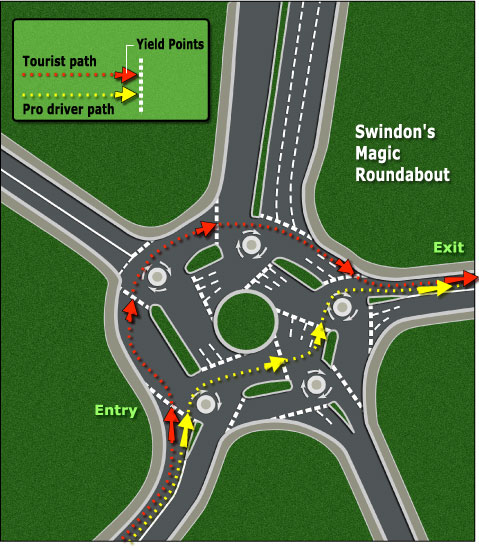
\includegraphics[scale=0.4]{images/itin}
			\caption{\label{itin} itinéraires possibles}
		\end{center}
	\end{figure}


\begin{figure}[p]
		\begin{center}
			\subfloat[le manège]{%
				\label{grman}
				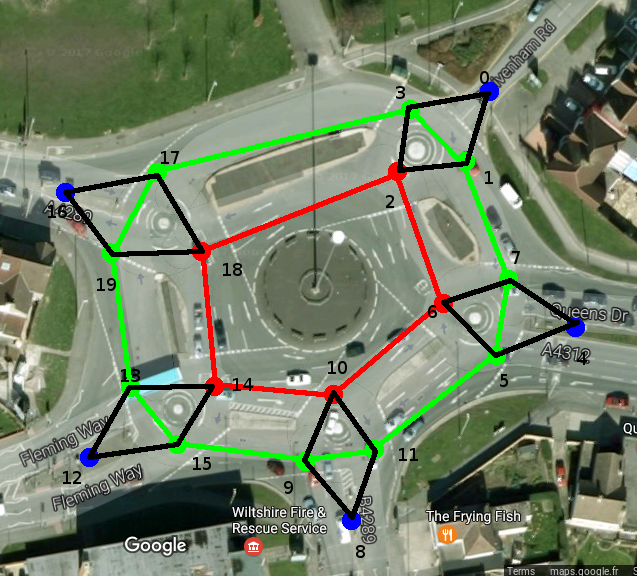
\includegraphics[scale=0.4]{../manege-graphe}
				}
			\subfloat[le rond-point]{%
				\label{grrp}
				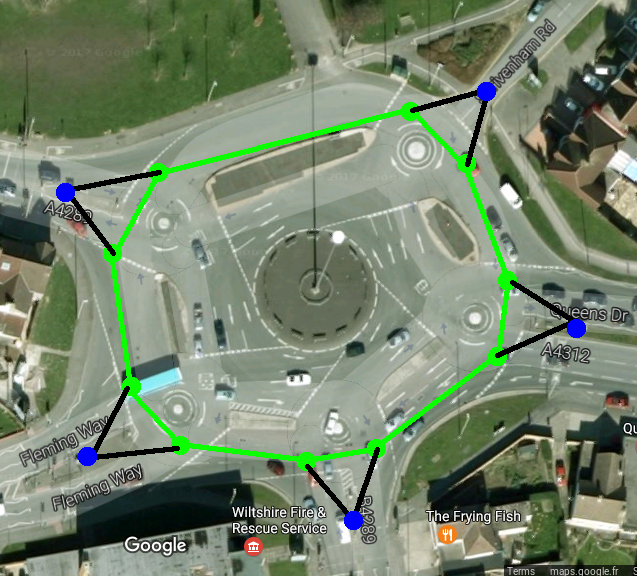
\includegraphics[scale=0.4]{../rp-graphe}}
		\end{center}	
		\caption{un graphe adapté au manège}
	\end{figure}


\begin{figure}[p]
	\begin{center}
		\caption{\label{rp}le manège enchanté}
		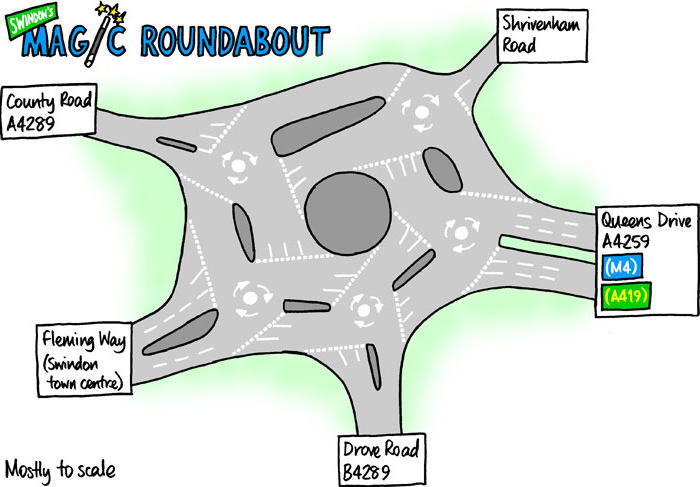
\includegraphics[scale=0.4]{images/magic-brit}
	\end{center}
\end{figure}



\begin{figure}[p]
	\begin{center}
	\begin{tabular}{ r|c c c c c}
  entrée & 0 & 4 & 8 & 12 & 16 \\ \hline
 0 & 21 & 100 & 100 & 60 & 36 \\
4 & 36 & 21 & 100 & 100 & 60 \\
8 & 60 & 36 & 21 & 100 & 100 \\
12 & 100 & 60 & 36 & 21 & 100 \\
16 & 100 & 100 & 60 & 36 & 21 \\
	\end{tabular}
	\end{center}
	\caption{\label{rpfw} Rapport entre la distance entrée-entrée pour le rond-point et le manège (en \%)}

\end{figure}


	\begin{figure}[hp]
		\begin{center}
			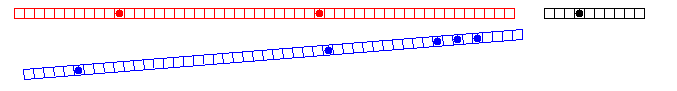
\includegraphics[scale=0.8]{./images/localdebut}
		\end{center}
		\caption{\label{locdeb}Un exemple d'intersection 2-1}
	\end{figure}


\begin{figure}[h]
	\begin{center}	
		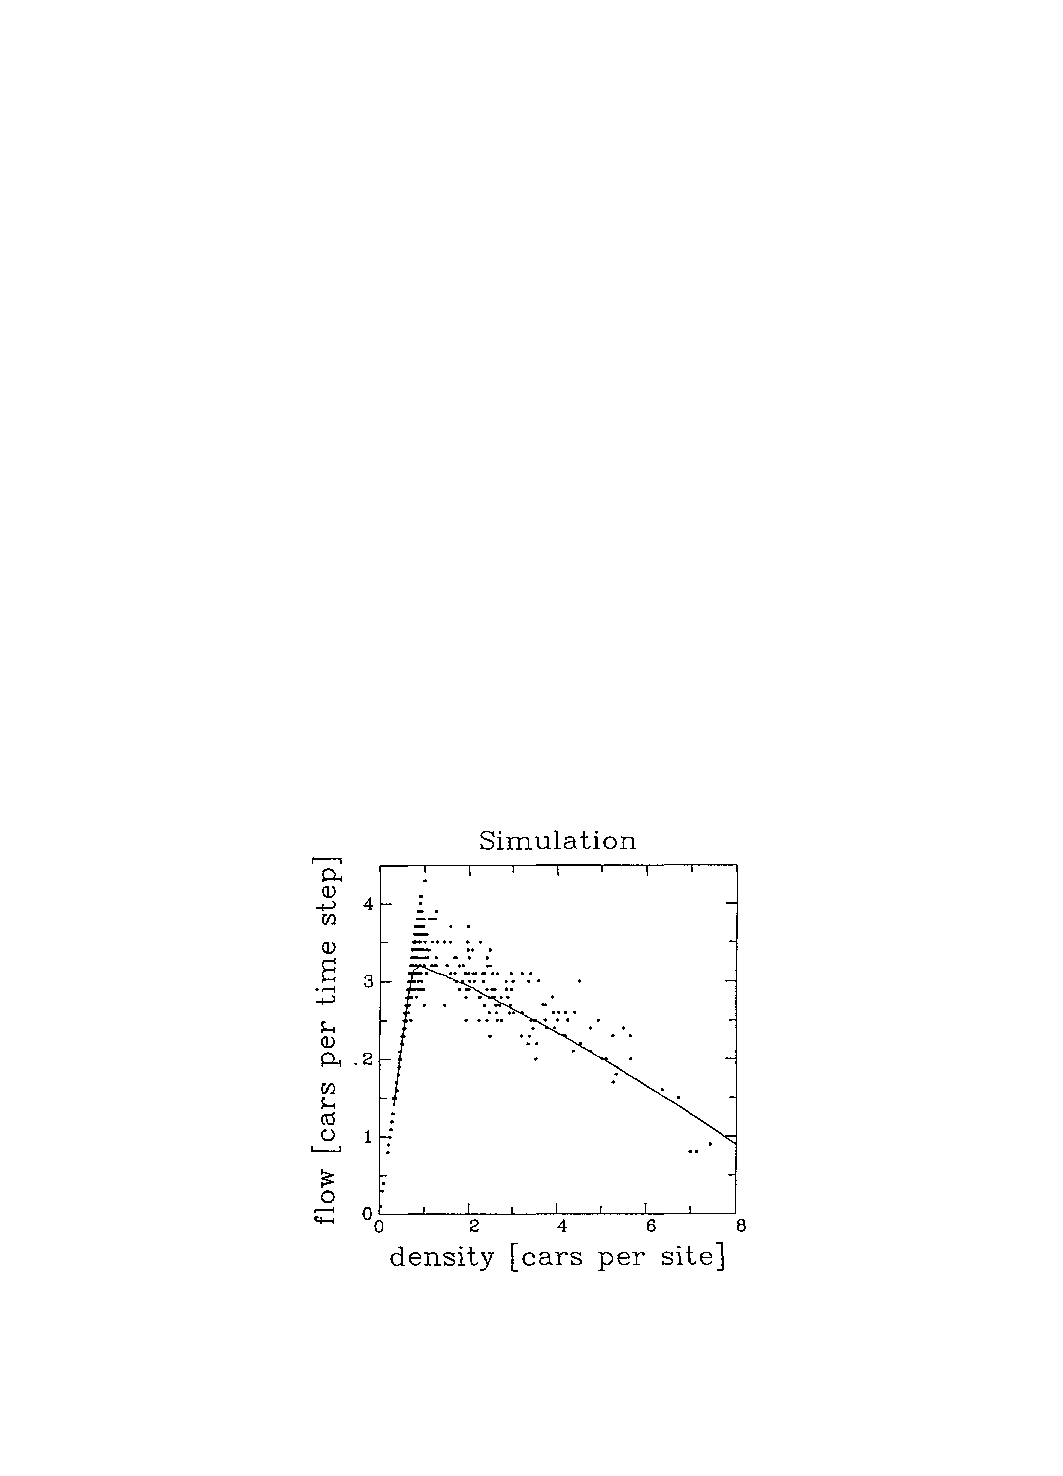
\includegraphics[scale = 1]{./images/dfondcomp}
	\end{center}
	\caption{\label{dgf} Un exemple de diagramme fondamental, tiré de \cite{NaSch}}
\end{figure}

	\begin{figure}[h]
		\begin{center}
			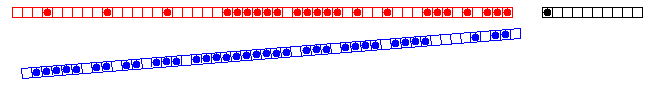
\includegraphics[scale=0.8]{./images/localsature}
		\end{center}
		\caption{\label{dsat}début de saturation}
	\end{figure}

	
\begin{figure}[h]
	\begin{center}
		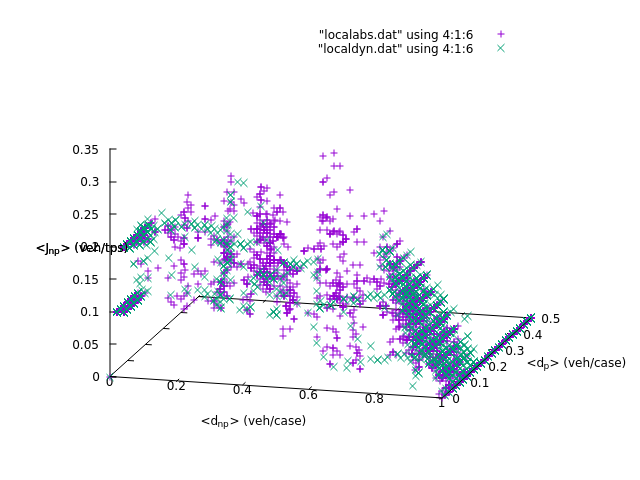
\includegraphics[scale=0.4]{./diagrammes-fondamentaux/localabsdyn0w}
	\end{center}
\caption{\label{prres}Comparaison absolu (en violet) / dynamique (en vert)}
\end{figure}	
	
\begin{figure}[h]
	 	\begin{center}
	 		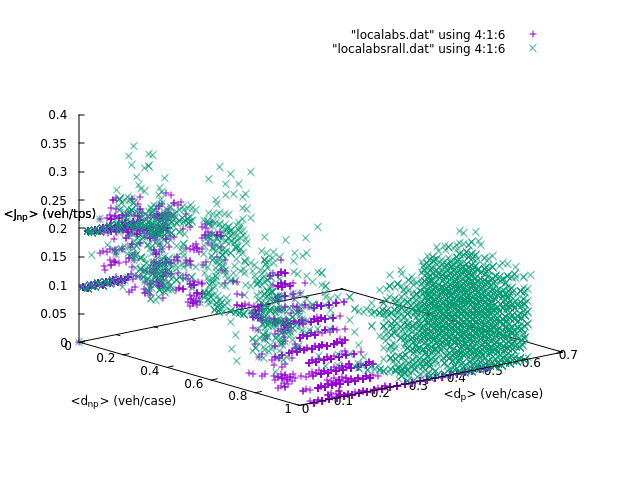
\includegraphics[scale=0.4]{./diagrammes-fondamentaux/localabs0w1w}
	 	\end{center}
	 	\caption{\label{rdem}Étude locale avec temps de démarrage}
	 	on observe une différence notable entre le modèle de priorité absolue sans temps de redémarrage (violet) et avec (vert)
	 \end{figure}

\begin{figure}[ht]
		\begin{center}
			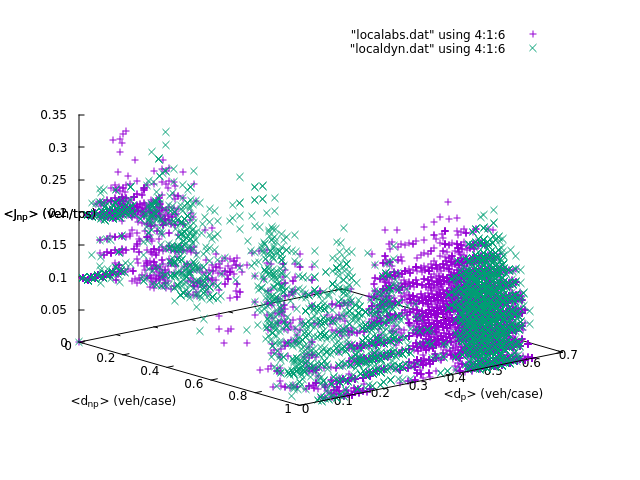
\includegraphics[scale=0.35]{./diagrammes-fondamentaux/localabsdyn1w}
		\end{center}
		\caption{\label{labstr}Comparaison absolu-dynamique pour un temps de réaction de 1}
\end{figure}
\end{document} 